\section{Part III: Nonlinear Dimensionality Reduction (for dataset B)}

Figure~\ref{fig:fig8} .....
\begin{figure}[htb]
 \centering
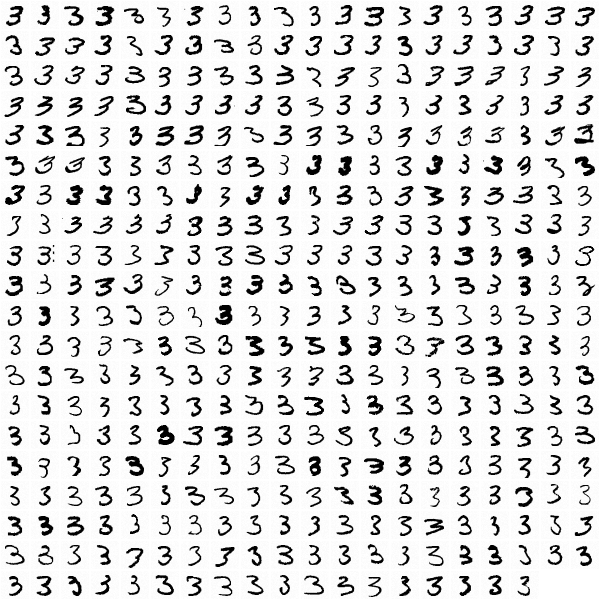
\includegraphics[width=4in]{assignment1/3-0-alldigit3.png}
\caption{\label{fig:fig8}figure caption}
\end{figure}


\clearpage{}
\subsection{Apply LLE to the images of digit '3' only}


Figure~\ref{fig:fig9} .....
\begin{figure}[htb]
 \centering
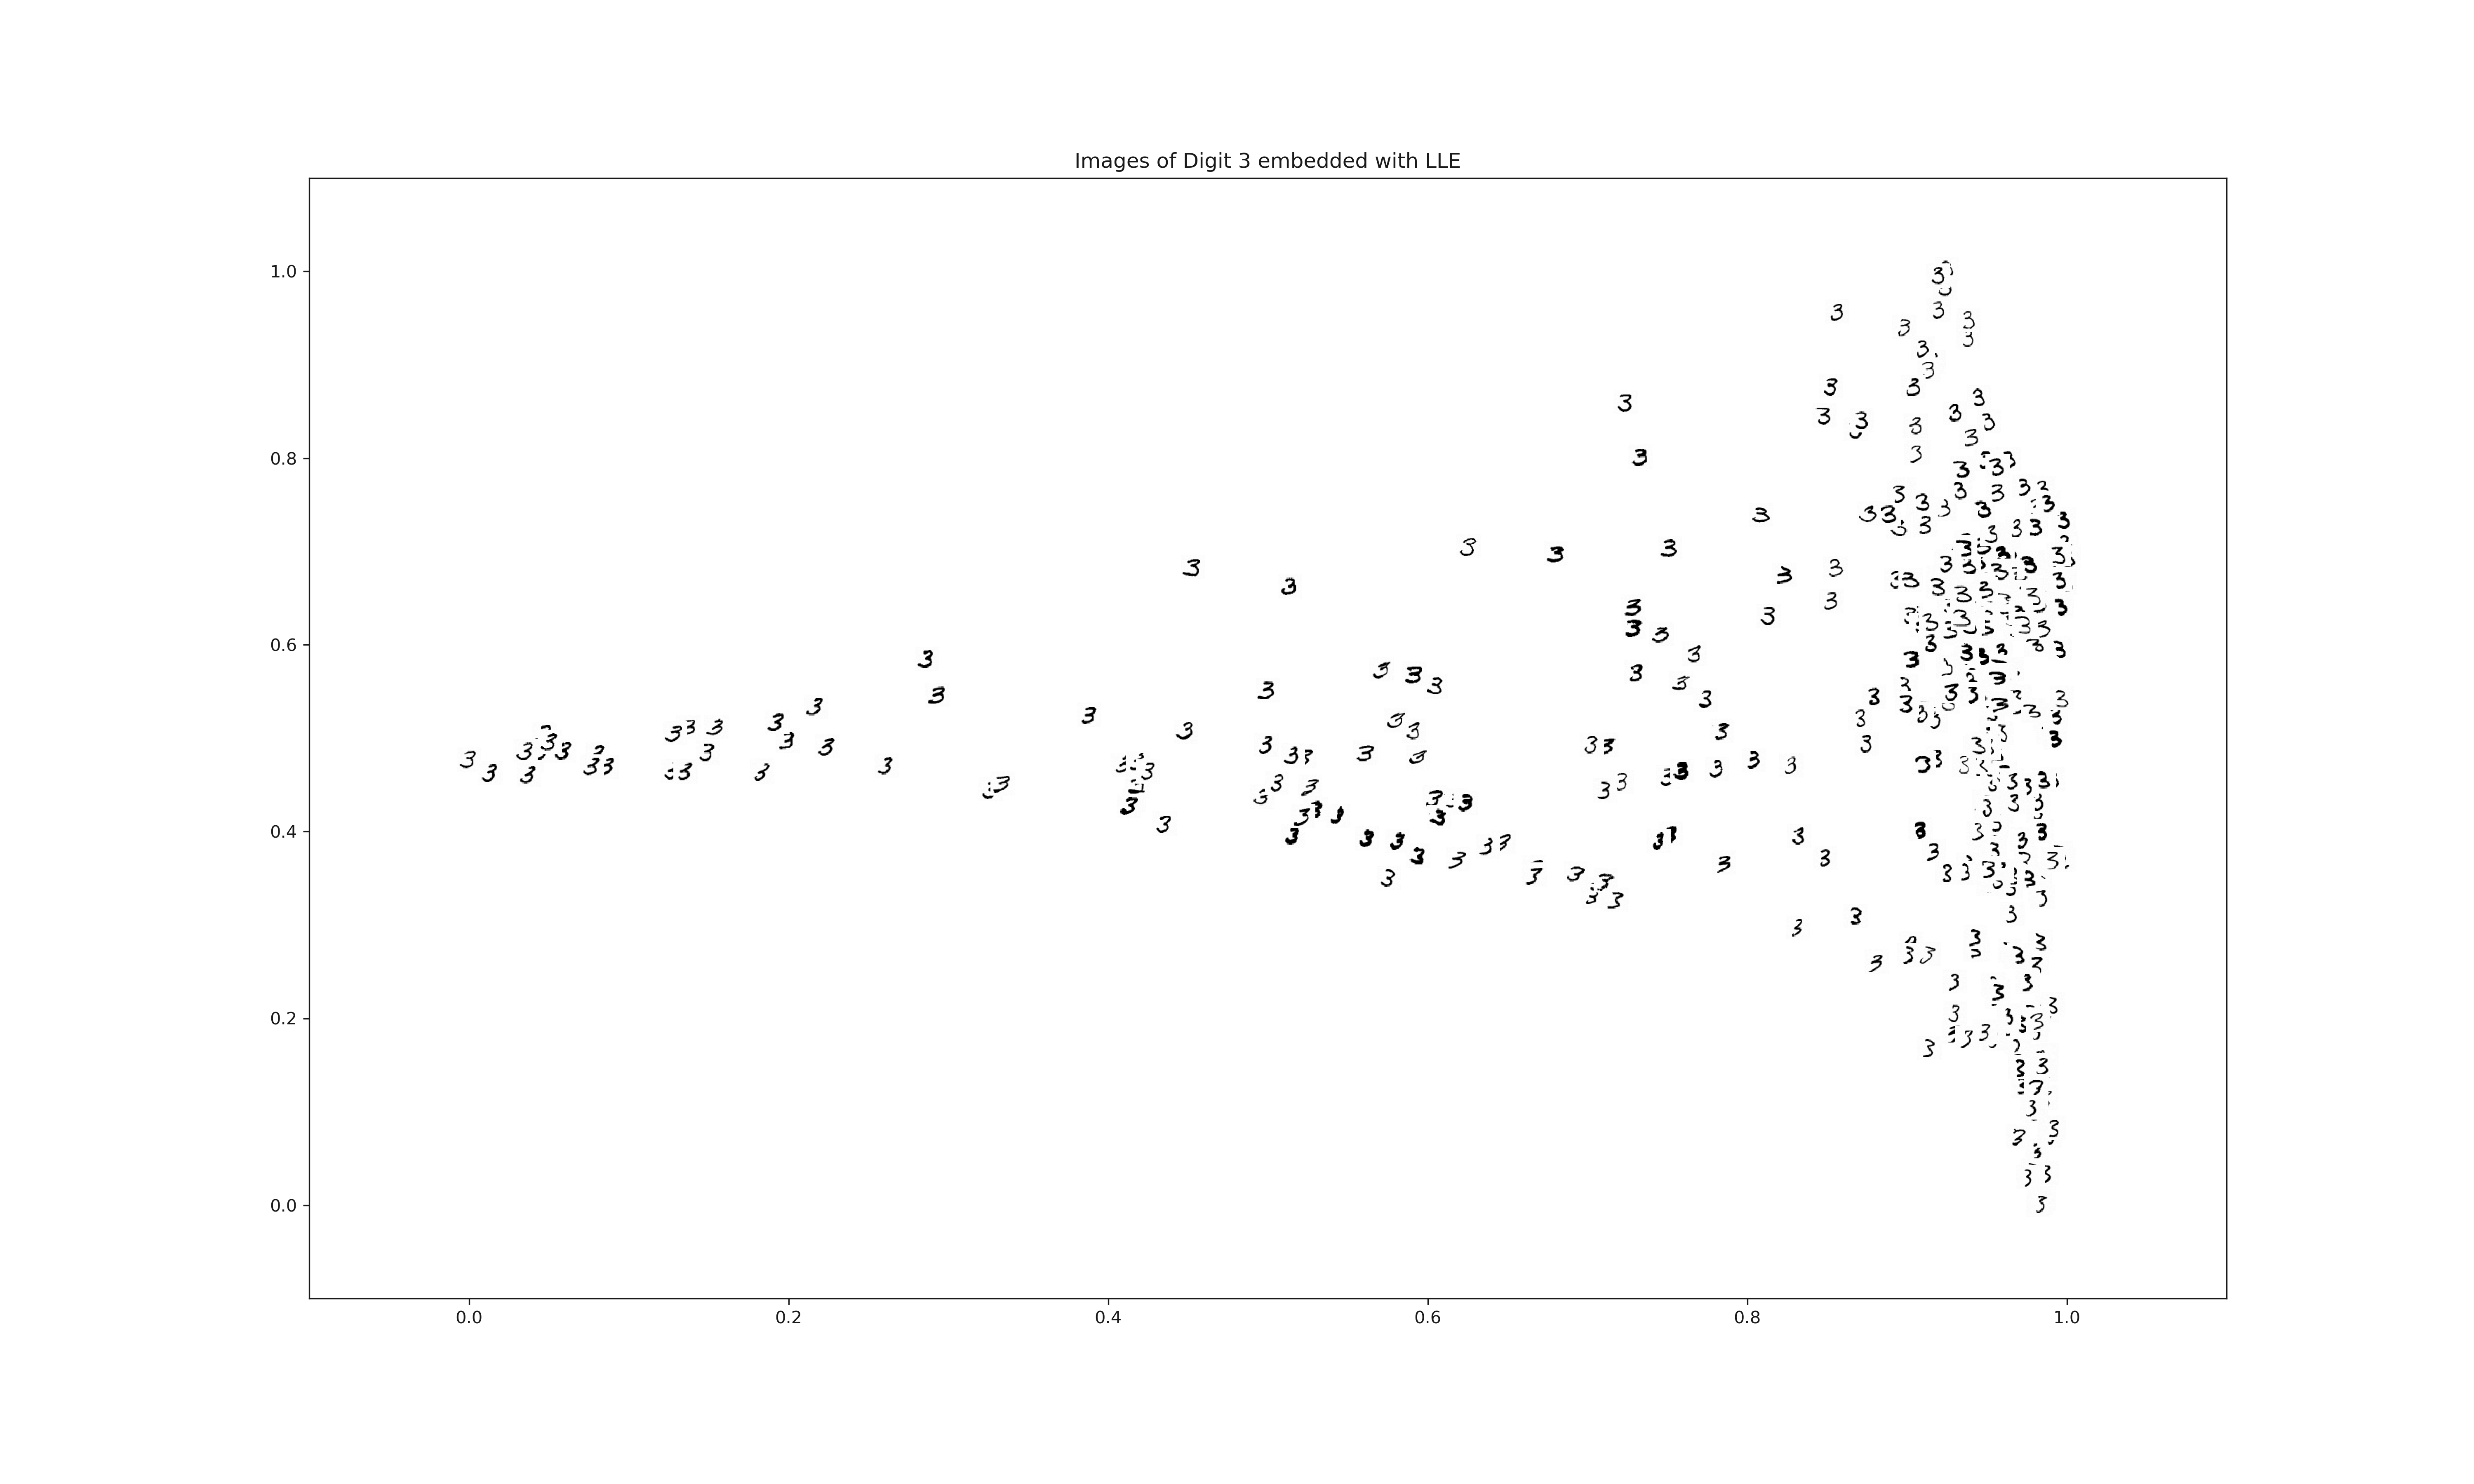
\includegraphics[width=\textwidth]{assignment1/3-1-LLEembedding.png}
\caption{\label{fig:fig9}figure caption}
\end{figure}



\clearpage{}
\subsection{Applying ISOMAP to the images of digit '3' only}

This is the beginning of the subsection.

Figure~\ref{fig:fig10} .....
\begin{figure}[htb]
 \centering
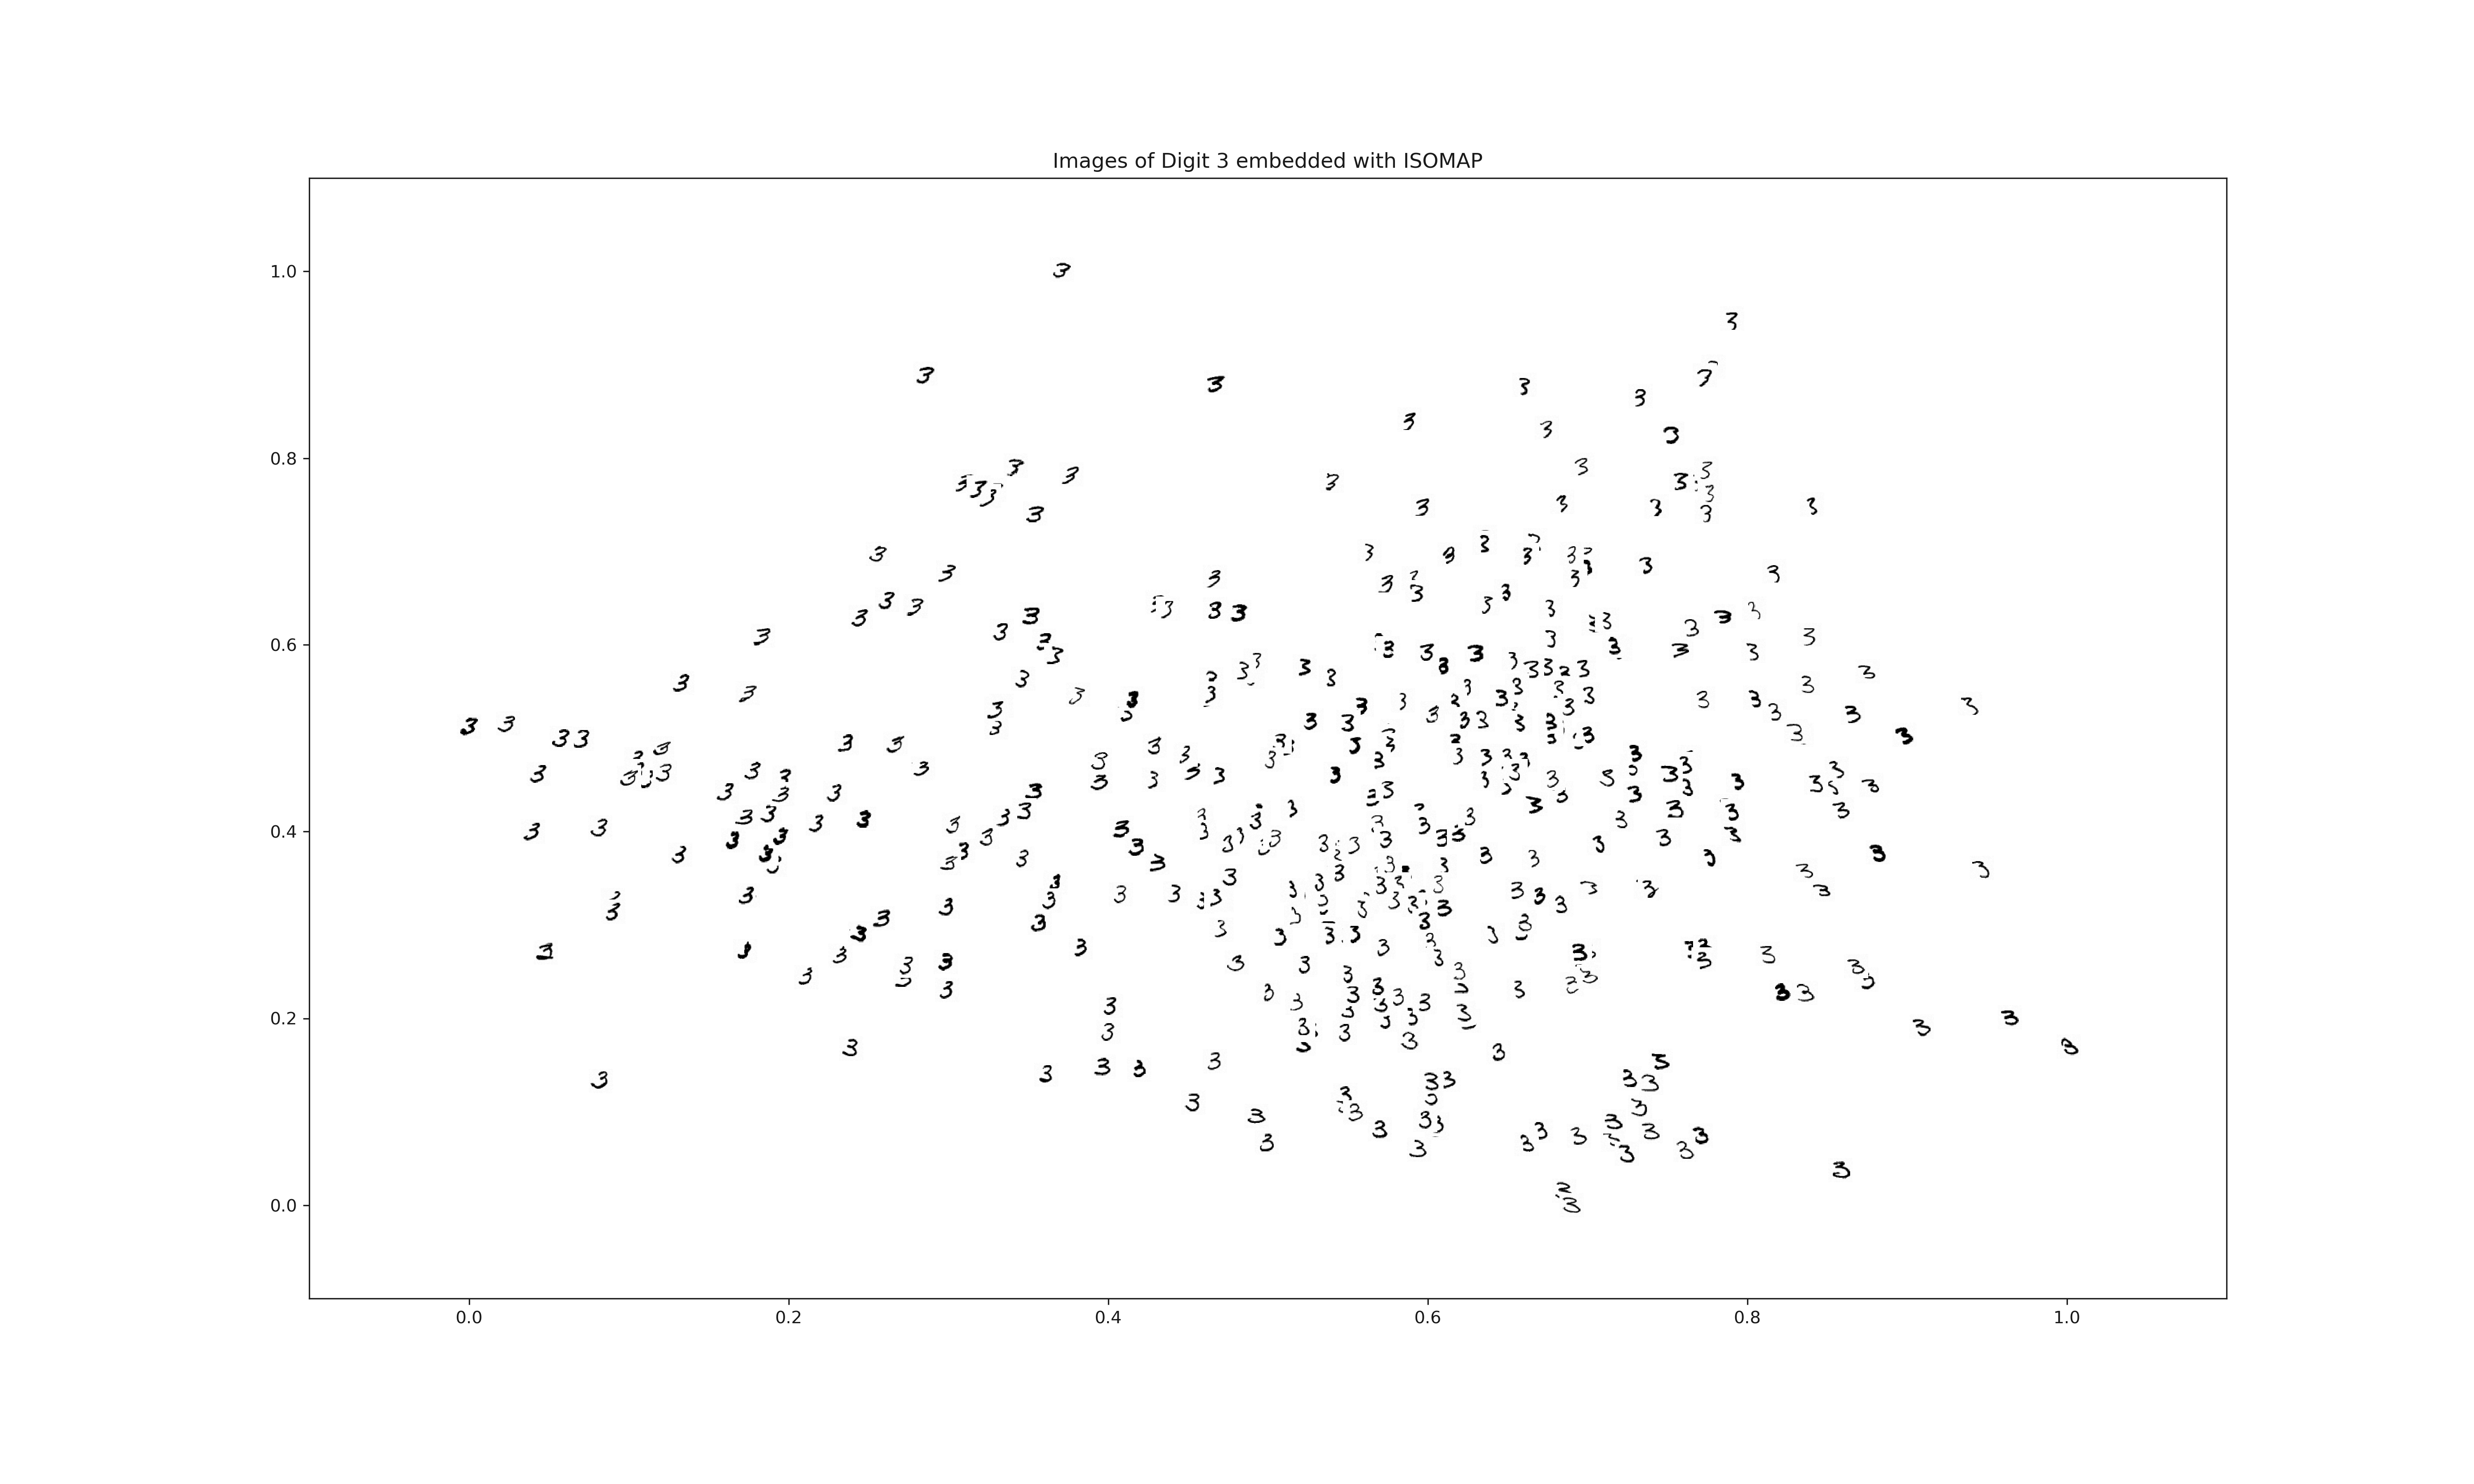
\includegraphics[width=\textwidth]{assignment1/3-2-ISOMAPembedding.png}
\caption{\label{fig:fig10}figure caption}
\end{figure}

\clearpage{}
\subsection{Naive Bayes classifier}

This is the beginning of the subsection.

